\subsection*{Teoria perturbativa indipendente dal tempo}
L'idea è che abbiamo una hamiltoniana $H$ che è la somma di una hamiltoniana $H_0$ imperturbata e una perturbazione $V'$:

\begin{equation*}
   H=H_0 + V'
\end{equation*}

Il motivo per cui indichiamo la perturbazione in tal modo è che in generale la hamiltoniana imperturbata potrebbe già avere parte del potenziale, cioè potrebbe essere nella forma $H_0=K + V$ con $K$ termine cinetico e $V$ termine di potenziale

Si parte dall'idea che noi conosciamo il sistema governato da $H_0$, quindi conosciamo sia i livelli di energia imperturbati $E_n^{(0)}$ che gli autostati $\ket*{n^{(0)}}$. In altri termini, conosciamo il problema

\begin{equation*}
   H_0\ket*{n^{(0)}}
   =E_n^{(0)}\ket*{n^{(0)}}
\end{equation*}

Quello che ci chiediamo è qual è la correzione ai livelli di energia imperturbati e agli autostati imperturbati a causa di $V'$. Omettendo i passaggi visti nella teoria, quello che andiamo a guardare negli esercizi in genere è al massimo il secondo ordine. La correzione al primo ordine è data dagli elementi di matrice del potenziale $V'$, sugli autostati imperturbati:

\begin{equation*}
   \delta E_n^{(1)}
   =E_n^{(1)} - E_n^{(0)}
   =\mel*{n^{(0)}}{V'}{n^{(0)}}
\end{equation*}

Per quanto riguarda la correzione al secondo ordine, essa è data da dall'elemento di matrice di $V'$ tra lo stato imperturbato $\ket*{n^{(0)}}$ e lo stato corretto al primo ordine $\ket*{n^{(1)}}$

\begin{equation*}
   \delta E_n^{(2)}
   =\mel*{n^{(0)}}{V'}{n^{(1)}}
\end{equation*}

Da tale espressione deduciamo che per avere una correzione all'ordine $n$-esimo ci servono gli autostati corretti fino all'ordine $n-1$. In particolare, per il secondo ordine ci serve lo stato corretto al primo ordine che è dato da

\begin{equation*}
   \ket*{n^{(1)}}
   =\sum_{k \neq n} \ket*{k^{(0)}} \frac{V'_{k,n}}{E_n^{(0)} - E_k^{(0)}}
   \qq{dove}
   V'_{k,n}=\mel*{k^{(0)}}{V'}{n^{(0)}}
\end{equation*}

Inserendo tale espressione in quella di sopra otteniamo

\begin{equation*}
   \delta E_n^{(2)}
   =\sum_{k \neq n} \frac{| \hspace{-0.1cm} \mel*{n^{(0)}}{V'}{k^{(0)}} \hspace{-0.1cm} |^2}{E_n^{(0)} - E_k^{(0)}}
\end{equation*}

Ci si può inoltre chiedere quando è valida la teoria perturbativa. Il criterio per stabilirlo è il seguente: il rapporto tra la correzione al primo ordine di un certo livello e la differenza tra l'energia del medesimo livello e quella del consecutivo deve essere molto minore di 1. In formule:

\begin{equation*}
   \biggl| \frac{\delta E_n^{(1)}}{ E_n^{(0)} - E_{n+1}^{(0)} } \biggr| \ll 1
\end{equation*}

\subsection*{Teoria perturbativa dipendente dal tempo}

Nella teoria perturbativa dipendente dal tempo consideriamo una hamiltoniana che ha un termine $H_0$ in cui non compare il tempo in maniera esplicita più un potenziale che dipende dal tempo:

\begin{equation*}
   H=H_0 + V(t)
\end{equation*}

In questo caso c'è un autostato $\ket{j}$ inizialmente popolato e la presenza del potenziale $V(t)$ può portare a delle transizioni verso uno stato $\ket*{n}$ con $n \neq j$. Uno degli scopi principali della teoria perturbativa dipendente dal tempo è quindi quello di calcolare qual è la probabilità di tale transizione. L'ampiezza della transizione $d_{j \to n}$ è data da

\begin{equation*}
   d_{j \to n}=-\frac{i}{\hbar} \int_{t_0}^{t} \dd{t'} e^{i \omega_{n,j} t'} V_{n,j}
\end{equation*}

dove

\begin{equation*}
   \omega_{n,j}=\frac{E_n - E_j}{\hbar}
   \qq{,}
   V_{n,j}=\mel*{n}{V(t)}{j}
\end{equation*}

L'integrale è esteso dal tempo $t_0$ in cui viene accesa la perturbazione fino al tempo $t$ in cui viene spenta.

\subsection*{Approssimazione WKB}

Tale approssimazione è molto utile quando vogliamo risolvere l'equazione di Schrödinger unidimensionale (o la parte radiale dell'equazione di Schrödinger nello spazio).

Essa considera il fatto che in generale possiamo avere un potenziale che varia debolmente (\textit{slowly-varing potential}) rispetto alla lunghezza d'onda della particella. Quindi, quando abbiamo tante lunghezze d'onda in questa regione e il potenziale varia poco, allora possiamo applicare la WKB. A differenza della teoria perturbativa che vale soltanto nel caso in cui la perturbazione è piccola, l'approssimazione WKB non necessita di questa richiesta: il potenziale può essere anche grande, ciò che conta è che vari lentamente.

\subsubsection*{Livelli di energia}
La WKB è utile per trovare i livelli di energia approssimati. Vediamo allora come si trovano. Considereremo principalmente tre casi:

\begin{enumerate}[leftmargin=0.6cm]
   \item Potenziale con due pareti verticali.
   
   Graficamente la situazione è la seguente, dove la regione classicamente permessa è quella compresa tra $x_1$ e $x_2$, mentre le regioni proibite sono rappresentato in grigio
   
   \begin{figure}[H]
      \centering
      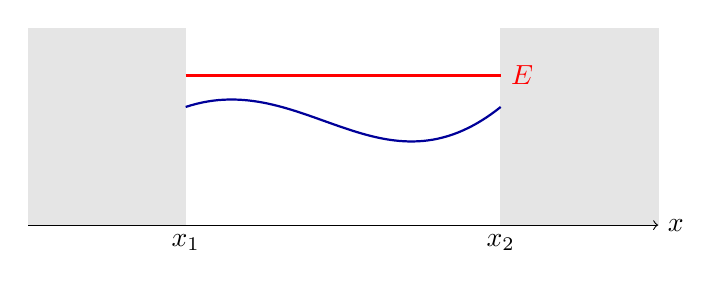
\begin{tikzpicture}
         \filldraw[gray!20!] (-2,0) node[black,below] {$x_1$} -- (-2,2.5) -- (-4,2.5) -- (-4,0) -- cycle;
         \filldraw[gray!20!] (2,0) node[black,below] {$x_2$} -- (2,2.5) -- (4,2.5) -- (4,0) -- cycle;
         \draw[->] (-4,0) -- (4,0) node[right] {$x$};
         \draw[thick,blue!60!black] (-2,1.5) .. controls (-0.5,2) and (0.5,0.3) .. (2,1.5);
         \draw[thick,red] (-2,1.9) -- (2,1.9) node[right] {$E$};
      \end{tikzpicture}
   \end{figure}

   Posto

   \begin{equation*}
      p=\sqrt{2m \bigl[ E - V(x) \bigr]}
   \end{equation*}

   Nel caso in cui $E>V$, possiamo trovare i livelli di energia risolvendo l'integrale:

   \begin{equation*}
      \int_{x_1}^{x_2} p(x) \dd{x}=n\pi\hbar
      \qq{,}
      n=1,2,\ldots
   \end{equation*}

   dove $x_1$ e $x_2$ sono i \textit{turning points} classici.
   \item Potenziale con una sola parete verticale.
   
   Supponendo di avere la parete verticale in $x_1$, dal punto di vista grafico la situazione è la seguente

   \begin{figure}[H]
      \centering
      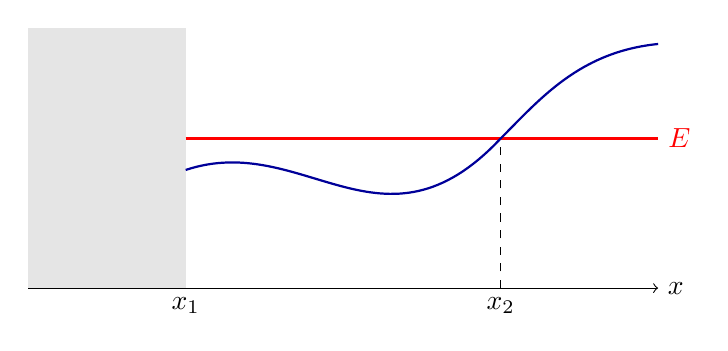
\begin{tikzpicture}
         \filldraw[gray!20!] (-2,0) node[black,below] {$x_1$} -- (-2,3.3) -- (-4,3.3) -- (-4,0) -- cycle;
         \draw[dashed] (2,0) node[black,below] {$x_2$} -- (2,1.9);
         \draw[->] (-4,0) -- (4,0) node[right] {$x$};
         \draw[red,thick] (-2,1.9) -- (4,1.9) node[right] {$E$};
         \draw[thick,blue!60!black] (-2,1.5) .. controls (-0.5,2) and (0.5,0.3) .. (2,1.9) .. controls (2.5,2.4) and (3,3) .. (4,3.1);
      \end{tikzpicture}
   \end{figure}

   Il secondo turning point si ha nel punto $x_2$, che dipende dal valore $E$ dell'energia, in quanto per trovarlo si impone la condizione $V(x_2)=E$. In questo caso, l'integrale da risolvere è\footnote{Attenzione! Si può utilizzare una formulazione differente in cui $n$ parte da $0$. In tal caso l'integrale da risolvere è
   \begin{equation*}
      \int_{x_1}^{x_2} p(x) \dd{x}=\qty( n + \frac{3}{4} )\pi\hbar
      \qq{,}
      n=0,1,\ldots
   \end{equation*}
   Per non confondersi, basta ricordare che per lo stato fondamentale si deve avere $\frac{3}{4}\pi\hbar$.}
   \begin{equation*}
      \int_{x_1}^{x_2} p(x) \dd{x}=\qty( n - \frac{1}{4} )\pi\hbar
      \qq{,}
      n=1,2,\ldots
   \end{equation*}
   
   \item Potenziale senza pareti verticali.
   In questo caso la situazione è la seguente:
   
   \begin{figure}[H]
      \centering
      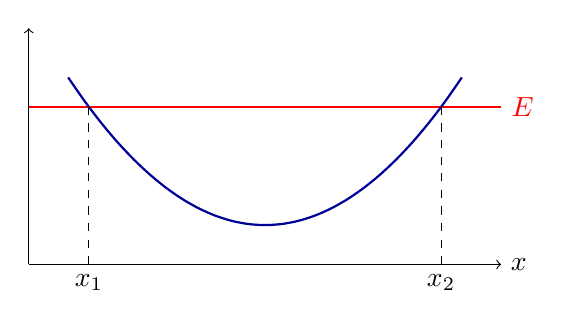
\begin{tikzpicture}
         \draw[->] (0,0) -- (6,0) node[right] {$x$};
         \draw[->] (0,0) -- (0,3);
         \draw[thick,red] (0,2) -- (6,2) node[right] {$E$};
         \draw[thick,blue!60!black!] plot[smooth,domain=-2.5:2.5] (\x+3,0.5+ 0.3*\x*\x);
         \draw[dashed] (5.236,0) node[below] {$x_2$} -- (5.236,2);
         \draw[dashed] (0.764,0) node[below] {$x_1$} -- (0.764,2);
      \end{tikzpicture}
   \end{figure}

   Attenzione! potrebbe capitare di avere un potenziale con una parete verticale, ma magari questa non è da considerare perché bisogna guardare dove l'energia eguaglia il potenziale. In altre parole, i turning points sono i punti $x_1, x_2$ tali che $V(x_{1,2})=E$.
   
   In questo caso, l'integrale da rivolvere per ottenere i livelli di energia approssimati è

   \begin{equation*}
      \int_{x_1}^{x_2} p(x) \dd{x}=\qty( n - \frac{1}{2} )\pi\hbar
      \qq{,}
      n=1,2,\ldots
   \end{equation*}

\end{enumerate}


\subsubsection*{Penetrabilità della barriera}

Nel caso in cui abbiamo una barriera di potenziale, la WKB può essere utilizzata per valutare la penetrabilità della barriera.

Per parlare di penetrabilità ci dobbiamo trovare nel caso $E<V$. Si ottiene che

\begin{equation*}
   T \simeq e^{-2\gamma}
   \qq{dove}
   \gamma=\frac{1}{\hbar} \int_{x_1}^{x_2} |p(x)| \dd{x}
\end{equation*}
dove $x_1$ e $x_2$ sono i classical turning points.

\subsection*{Scattering Theory}
Nella teoria dello scattering studiamo sistemi in cui c'è una regione dello spazio con un certo potenziale $V$ avente un certo range $R_V$ e abbiamo un'onda piana incidente. Il risultato dell'interazione tra questa e il potenziale è un'onda piana uscente più un'onda sferica:
\begin{equation*}
   \psi(x)=\varphi_k(x) - \frac{2m}{\hbar^2} \frac{e^{i k r}}{r} f(\vb{k}, \vb{k'})
\end{equation*}
L'obiettivo della teoria dello scattering è determinare l'ampiezza di scattering $f(\vb{k}, \vb{k'})$, da cui possiamo ottenere la sezione d'urto differenziale, definita come
\begin{equation*}
   \dv{\sigma}{\Omega}
   =| f(\vb{k}, \vb{k'}) |^2
\end{equation*}
e da cui a sua volta si può ottenere la sezione d'urto totale integrando su tutto l'angolo solido.
\subsubsection*{Approssimazione di Born}
Un primo metodo per risolvere il problema dello scattering è quello dell'approssimazione di Born al primo ordine. Con tale metodo si trova che la sezione d'urto di Born è
\begin{equation*}
   f^{\rm Born}(\vb{k}, \vb{k'})
   =-\frac{1}{4 \pi} \frac{2 m}{\hbar^2} \int \dd[3]{x} e^{i (\vb{k} - \vb{k}') \vdot \vb{x}} V(\vb{x})
\end{equation*}
Spesso si preferisce esprimere tale quantità in termini del momento trasferito $\vb{q}=\vb{k} - \vb{k'}$:\footnote{Attenzione! In alcuni testi si potrebbe trovare la formula con un segno meno nell'esponenziale. Ciò è dovuto al fatto che in essi il momento trasferito è stato definito come $q=k'-k$.}
\begin{equation*}
   f^{\rm Born}(\vb{k}, \vb{k'})
   =-\frac{m}{2 \pi \hbar^3} \int \dd[3]{x} e^{i \vb{q} \vdot \vb{x}} V(\vb{x})
\end{equation*}
e tale espressione risulta essere la trasformata di Fourier del potenziale $V(\vb{x})$.\\
Nel caso di potenziali centrali, in cui $V(\vb{x}) \equiv V(r)$, la sezione d'urto differenziale si può esprimere come
\begin{equation*}
   f^{\rm Born}(\vartheta)
   =-\frac{2m}{\hbar^2} \int_{0}^{\infty} \dd{r} r V(r) \frac{\sin{(qr)}}{q}
\end{equation*}
Inoltre si può dimostrare che il modulo del momento trasferito è $q=2k \sin(\vartheta/2)$, dove $\vartheta$ è l'angolo di scattering tra $\vb{k}$ e $\vb{k'}$.
%\subsubsection*{Partial wave expansion}